\section{Lesson 14 --- 12/11/2026}

\subsection{Clustering problems}

In classification and regression each pattern comes with a label or a value to predict. We now consider the case in which the data have no labels and we want to group the patterns according to their similarity.

\begin{definition}[Clustering problem]
Given a set $S$ of patterns and an integer number $k$, a \g{clustering problem} consists in finding a partition of $S$ in $k$ subsets $S_1,\dots,S_k$ (\g{clusters}) that are homogeneous and well separated.
\end{definition}

Clustering problems are an example of unsupervised machine learning methods.

\subsubsection{The optimization model}

To turn the definition into an optimization problem we need a way to measure how homogeneous a cluster is. We do it with a distance and a representative point for each cluster:

\begin{itemize}
    \item Assume that patterns are vectors $p^1,\dots,p^\ell \in \R^n$.
    \item Consider a distance $d \colon \R^n \times \R^n \to \R$ between vectors in $\R^n$. In what follows we will consider the square distance $d(x,y) = \norm{x-y}_2^2$ or $d(x,y) = \norm{x-y}_1$.
    \item For each cluster $S_j$ introduce a \g{centroid} $x^j \in \R^n$ (unknown).
    \item Define clusters so that each pattern is associated to the closest centroid.
\end{itemize}
We aim to find $k$ centroids in order to minimize the sum of the distances between each pattern and the closest centroid. The model is
\[
\begin{cases}
\displaystyle \min \sum_{i=1}^{\ell} \min_{j=1,\dots,k} d(p^i, x^j)\\[1ex]
x^j \in \R^n & \forall\, j=1,\dots,k.
\end{cases}
\]

\subsubsection{The optimization model with \texorpdfstring{$\norm{\cdot}_2$}{the 2-norm}}

Consider the square distance $d(x,y) = \norm{x-y}_2^2$. The optimization problem to solve is
\[
\begin{cases}
\displaystyle \min \sum_{i=1}^{\ell} \min_{j=1,\dots,k} \norm{p^i - x^j}_2^2\\[1ex]
x^j \in \R^n & \forall\, j=1,\dots,k.
\end{cases}
\]

We start from the simplest case. If $k=1$ (one cluster), then it is a convex quadratic programming problem without constraints:
\begin{equation}\label{eq:clust-one}
\begin{cases}
\displaystyle \min \sum_{i=1}^{\ell} \norm{p^i - x}_2^2 = \min \sum_{i=1}^{\ell} (x-p^i)^T(x-p^i)\\[1ex]
x \in \R^n.
\end{cases}
\end{equation}
The global optimum is the stationary point:
\[
2\ell x - 2\sum_{i=1}^{\ell} p^i = 0 \quad\Longleftrightarrow\quad x = \frac{\sum_{i=1}^{\ell} p^i}{\ell} \qquad \text{(mean or barycenter)}.
\]

If $k>1$ (at least two clusters), then the problem is nonconvex and nondifferentiable:
\begin{equation}\label{eq:clust-nonconvex}
\begin{cases}
\displaystyle \min_{x} \sum_{i=1}^{\ell} \min_{j=1,\dots,k} \norm{p^i - x^j}_2^2\\[1ex]
x^j \in \R^n & \forall\, j=1,\dots,k.
\end{cases}
\end{equation}
The nondifferentiability comes from the inner minimum over $j$. The idea is to get rid of it by introducing new variables. We observe that, for fixed $p^i$ and $x^j$, $j=1,\dots,k$,
\begin{equation}\label{eq:clust-alpha}
\min_{j=1,\dots,k} \norm{p^i - x^j}_2^2 =
\begin{cases}
\displaystyle \min \sum_{j=1}^{k} \alpha_{ij}\norm{p^i - x^j}_2^2\\[1ex]
\displaystyle \sum_{j=1}^{k} \alpha_{ij} = 1\\[1ex]
\alpha_{ij} \ge 0 & \forall\, j=1,\dots,k,
\end{cases}
\end{equation}
where the variables in \eqref{eq:clust-alpha} are $\alpha_{i1},\alpha_{i2},\dots,\alpha_{ik}$.

\begin{remark}
It is enough to notice that, fixed scalars $a_1,a_2,\dots,a_k$, we have that
\[
\min_{j=1,\dots,k} \{a_j\} = \min\left\{ \sum_{j=1}^{k} \alpha_j a_j \;:\; \sum_{j=1}^{k} \alpha_j = 1,\ \alpha \ge 0 \right\}.
\]
\end{remark}

An optimal solution of \eqref{eq:clust-alpha} is given by
\begin{equation}\label{eq:clust-alpha-opt}
\alpha_{ij}^* =
\begin{cases}
1 & \text{if } \norm{p^i - x^j}_2 = \min\limits_{h=1,\dots,k} \norm{p^i - x^h}_2\\
0 & \text{otherwise.}
\end{cases}
\end{equation}

\begin{remark}
Observe that $\alpha_{ij}^* = 1$ if pattern $i$ is assigned to cluster $j$.
\end{remark}

Replacing each inner minimum in \eqref{eq:clust-nonconvex} with \eqref{eq:clust-alpha}, the $\alpha_{ij}$ become additional variables of the problem and the objective function becomes differentiable.

\begin{theorem}
Problem \eqref{eq:clust-nonconvex} is equivalent to the following nonconvex differentiable problem:
\begin{equation}\label{eq:clust-diff}
\begin{cases}
\displaystyle \min_{x,\alpha} f(x,\alpha) := \sum_{i=1}^{\ell}\sum_{j=1}^{k} \alpha_{ij}\norm{p^i - x^j}_2^2\\[1ex]
\displaystyle \sum_{j=1}^{k} \alpha_{ij} = 1 & \forall\, i=1,\dots,\ell\\[1ex]
\alpha_{ij} \ge 0 & \forall\, i=1,\dots,\ell,\ j=1,\dots,k\\
x^j \in \R^n & \forall\, j=1,\dots,k.
\end{cases}
\end{equation}
\end{theorem}

\subsubsection{The \texorpdfstring{$k$}{k}-means algorithm}

Problem \eqref{eq:clust-diff} is hard to solve jointly in $(x,\alpha)$, but it becomes easy when one of the two blocks of variables is fixed. The \g{$k$-means algorithm} is based on the following properties of problem \eqref{eq:clust-diff}:
\begin{itemize}
    \item If $x^j$ are fixed, then \eqref{eq:clust-diff} is decomposable into $\ell$ simple LP problems of the form \eqref{eq:clust-alpha}: for any $i=1,\dots,\ell$, the optimal solution is
    \[
    \alpha_{ij}^* =
    \begin{cases}
    1 & \text{if } j \text{ is the first index s.t. } \norm{p^i - x^j}_2 = \min\limits_{h=1,\dots,k} \norm{p^i - x^h}_2\\
      & \text{($x^j$ is the first closest centroid to $p^i$),}\\
    0 & \text{otherwise.}
    \end{cases}
    \]
    \item If $\alpha_{ij}$ are fixed, then \eqref{eq:clust-diff} is decomposable into $k$ convex QP problems (in the unknown $x^j$) similar to \eqref{eq:clust-one}, i.e.,
    \begin{equation}\label{eq:clust-centroid}
    \begin{cases}
    \displaystyle \min \sum_{i=1}^{\ell} \alpha_{ij}\norm{p^i - x^j}_2^2 = \min \sum_{i=1}^{\ell} \alpha_{ij}(x^j-p^i)^T(x^j-p^i)\\[1ex]
    x^j \in \R^n.
    \end{cases}
    \end{equation}
    For any $j=1,\dots,k$, the optimal solution of \eqref{eq:clust-centroid} is
    \[
    (x^j)^* = \frac{\sum_{i=1}^{\ell} \alpha_{ij}\, p^i}{\sum_{i=1}^{\ell} \alpha_{ij}} \qquad \text{(mean of patterns).}
    \]
\end{itemize}

The $k$-means algorithm consists in an alternating minimization of
\[
f(x,\alpha) = \sum_{i=1}^{\ell}\sum_{j=1}^{k} \alpha_{ij}\norm{p^i - x^j}_2^2
\]
with respect to the two blocks of variables $x$ and $\alpha$. We denote by $x^{j,t}$ and $\alpha_{ij}^t$ the centroids and the assignments at iteration $t$.

\begin{algorithm}[H]
\caption{$k$-means algorithm}
Set $t = 0$, choose centroids $x^{1,0},\dots,x^{k,0} \in \R^n$\;
\For(\tcp*[f]{assign patterns to clusters}){$i=1,\dots,\ell$}{
    $\alpha_{ij}^0 = \begin{cases} 1 & \text{if } j \text{ is the first index s.t. } \norm{p^i - x^{j,0}}_2 = \min\limits_{h=1,\dots,k} \norm{p^i - x^{h,0}}_2\\ 0 & \text{otherwise}\end{cases}$\;
}
\While{true}{
    \For(\tcp*[f]{update centroids}){$j=1,\dots,k$}{
        $x^{j,t+1} = \left(\sum_{i=1}^{\ell} \alpha_{ij}^t\, p^i\right) \Big/ \left(\sum_{i=1}^{\ell} \alpha_{ij}^t\right)$\;
    }
    \For(\tcp*[f]{update clusters}){$i=1,\dots,\ell$}{
        $\alpha_{ij}^{t+1} = \begin{cases} 1 & \text{if } j \text{ is the first index s.t. } \norm{p^i - x^{j,t+1}}_2 = \min\limits_{h=1,\dots,k} \norm{p^i - x^{h,t+1}}_2\\ 0 & \text{otherwise}\end{cases}$\;
    }
    \eIf(\tcp*[f]{stopping criterion}){$f(x^{t+1},\alpha^{t+1}) = f(x^t,\alpha^t)$}{
        STOP\;
    }{
        $t = t+1$\;
    }
}
\end{algorithm}

Since each step is a minimization with respect to one block of variables, the value of $f$ never increases along the iterations. This leads to the following convergence result.

\begin{theorem}
The $k$-means algorithm stops after a finite number of iterations at a solution $(x^*,\alpha^*)$ of the KKT system of problem \eqref{eq:clust-diff} such that
\begin{align*}
f(x^*,\alpha^*) &\le f(x^*,\alpha) && \forall\, \alpha \ge 0 \text{ s.t. } \sum_{j=1}^{k} \alpha_{ij} = 1 \quad \forall\, i=1,\dots,\ell,\\
f(x^*,\alpha^*) &\le f(x,\alpha^*) && \forall\, x \in \R^{kn}.
\end{align*}
\end{theorem}

\begin{remark}
The $k$-means algorithm does not guarantee to find a global optimum.
\end{remark}

\subsubsection{The optimization model with \texorpdfstring{$\norm{\cdot}_1$}{the 1-norm}}

We now repeat the same analysis with a different distance. Consider the distance $d(x,y) = \norm{x-y}_1$. The optimization problem to solve is
\[
\begin{cases}
\displaystyle \min \sum_{i=1}^{\ell} \min_{j=1,\dots,k} \norm{p^i - x^j}_1\\[1ex]
x^j \in \R^n & \forall\, j=1,\dots,k.
\end{cases}
\]

As before, we start from the simplest case. If $k=1$ (one cluster), then it is a convex problem decomposable into $n$ convex problems of one variable:
\begin{equation}\label{eq:clust-l1-one}
\begin{cases}
\displaystyle \min \sum_{i=1}^{\ell} \norm{p^i - x}_1 = \min \sum_{i=1}^{\ell}\sum_{h=1}^{n} \lvert x_h - p^i_h \rvert = \min \sum_{h=1}^{n} \underbrace{\sum_{i=1}^{\ell} \lvert x_h - p^i_h \rvert}_{f_h(x_h)}\\[1ex]
x \in \R^n,
\end{cases}
\end{equation}
where $x_h$ and $p^i_h$ denote the $h$-th components of $x$ and $p^i$. Each $f_h$ depends only on the component $x_h$, so the $n$ functions can be minimized separately. We are left with the following question: given $\ell$ real numbers $a_1 < a_2 < \dots < a_\ell$, what is the optimal solution of
\[
\begin{cases}
\displaystyle \min \sum_{i=1}^{\ell} \lvert x - a_i \rvert = f(x)\\[1ex]
x \in \R \,?
\end{cases}
\]
The objective function is convex and piecewise linear:
\[
f(x) =
\begin{cases}
-\ell x + \sum_{i=1}^{\ell} a_i & \text{if } x < a_1\\
(2-\ell)x + \sum_{i=2}^{\ell} a_i - a_1 & \text{if } x \in [a_1,a_2]\\
\quad\vdots & \quad\vdots\\
(2r-\ell)x + \sum_{i=r+1}^{\ell} a_i - \sum_{i=1}^{r} a_i & \text{if } x \in [a_r,a_{r+1}]\\
\quad\vdots & \quad\vdots\\
(\ell-2)x + a_\ell - \sum_{i=1}^{\ell-1} a_i & \text{if } x \in [a_{\ell-1},a_\ell]\\
\ell x - \sum_{i=1}^{\ell} a_i & \text{if } x > a_\ell.
\end{cases}
\]
The slope $2r-\ell$ increases with $r$: it is negative as long as $r < \ell/2$ and positive when $r > \ell/2$, so $f$ decreases up to the middle of the points and increases afterwards. Hence the global optimum is
\[
\operatorname{median}(a_1,\dots,a_\ell) =
\begin{cases}
a_{(\ell+1)/2} & \text{if $\ell$ is odd,}\\[1ex]
\dfrac{a_{\ell/2} + a_{1+\ell/2}}{2} & \text{if $\ell$ is even.}
\end{cases}
\]

\begin{remark}
If $\ell$ is even, the slope of $f$ is zero on $[a_{\ell/2}, a_{1+\ell/2}]$, hence every point of this interval is a global optimum and the median is its midpoint.
\end{remark}

\begin{example}
\leavevmode
\begin{enumerate}[label=(\alph*)]
    \item $f(x) = \lvert x-2 \rvert + \lvert x-4 \rvert + \lvert x-10 \rvert$, $\ell = 3$. The global optimum is $\operatorname{median}(2,4,10) = a_{(\ell+1)/2} = a_2 = 4$.
    \item $f(x) = \lvert x-2 \rvert + \lvert x-4 \rvert + \lvert x-6 \rvert + \lvert x-10 \rvert$, $\ell = 4$. The global optimum is $\operatorname{median}(2,4,6,10) = \dfrac{a_{\ell/2} + a_{1+\ell/2}}{2} = \dfrac{4+6}{2} = 5$.
\end{enumerate}
\begin{center}
\begin{tikzpicture}
\begin{axis}[width=0.48\textwidth, height=5cm, xmin=-2, xmax=14, ymin=0, axis lines=left, xtick={2,4,10}, title={(a)}, title style={font=\small}, tick label style={font=\small}]
\addplot[blue, thick, domain=-2:14, samples at={-2,2,4,10,14}] {abs(x-2)+abs(x-4)+abs(x-10)};
\addplot[only marks, mark=*, red] coordinates {(4,8)};
\end{axis}
\end{tikzpicture}
\hfill
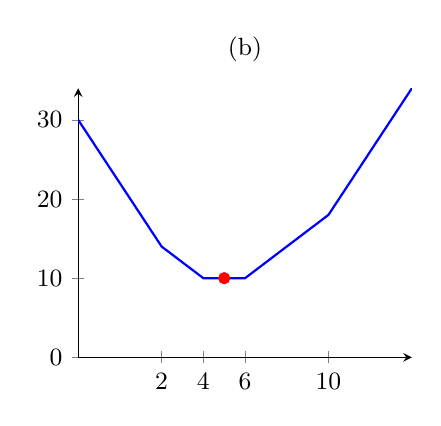
\begin{tikzpicture}
\begin{axis}[width=0.48\textwidth, height=5cm, xmin=-2, xmax=14, ymin=0, axis lines=left, xtick={2,4,6,10}, title={(b)}, title style={font=\small}, tick label style={font=\small}]
\addplot[blue, thick, domain=-2:14, samples at={-2,2,4,6,10,14}] {abs(x-2)+abs(x-4)+abs(x-6)+abs(x-10)};
\addplot[only marks, mark=*, red] coordinates {(5,10)};
\end{axis}
\end{tikzpicture}
\end{center}
\end{example}

Going back to \eqref{eq:clust-l1-one}, the optimal solution for $k=1$ is the vector whose $h$-th component is the median of the $h$-th components of the patterns, i.e., the componentwise median of $p^1,\dots,p^\ell$.

If $k>1$ (at least two clusters), then the problem is nonconvex and nonsmooth:
\begin{equation}\label{eq:clust-l1}
\begin{cases}
\displaystyle \min_{x} \sum_{i=1}^{\ell} \min_{j=1,\dots,k} \norm{p^i - x^j}_1\\[1ex]
x^j \in \R^n & \forall\, j=1,\dots,k.
\end{cases}
\end{equation}
The inner minimum over $j$ can be removed with the same variables $\alpha_{ij}$ used for the square distance.

\begin{theorem}
Problem \eqref{eq:clust-l1} is equivalent to the following problem:
\begin{equation}\label{eq:clust-l1-alpha}
\begin{cases}
\displaystyle \min_{x,\alpha} \sum_{i=1}^{\ell}\sum_{j=1}^{k} \alpha_{ij}\norm{p^i - x^j}_1\\[1ex]
\displaystyle \sum_{j=1}^{k} \alpha_{ij} = 1 & \forall\, i=1,\dots,\ell\\[1ex]
\alpha_{ij} \ge 0 & \forall\, i=1,\dots,\ell,\ j=1,\dots,k\\
x^j \in \R^n & \forall\, j=1,\dots,k.
\end{cases}
\end{equation}
\end{theorem}

Differently from \eqref{eq:clust-diff}, the objective function of \eqref{eq:clust-l1-alpha} is still nondifferentiable, because of the absolute values in the 1-norm. Note that
\[
f(x,\alpha) := \sum_{i=1}^{\ell}\sum_{j=1}^{k} \alpha_{ij}\norm{p^i - x^j}_1 = \sum_{i=1}^{\ell}\sum_{j=1}^{k}\sum_{h=1}^{n} \alpha_{ij}\, u_{ijh},
\]
where we set
\[
u_{ijh} = \lvert x^j_h - p^i_h \rvert = \max\{x^j_h - p^i_h,\ p^i_h - x^j_h\}.
\]
Since $\alpha_{ij} \ge 0$ and we are minimizing, each $u_{ijh}$ can be treated as a new variable bounded from below by the two terms of the maximum. Consequently, we have the following result.

\begin{theorem}
Problem \eqref{eq:clust-l1-alpha} is equivalent to the nonconvex differentiable (bilinear) problem:
\[
\begin{cases}
\displaystyle \min_{x,\alpha,u} \sum_{i=1}^{\ell}\sum_{j=1}^{k}\sum_{h=1}^{n} \alpha_{ij}\, u_{ijh}\\[1ex]
u_{ijh} \ge p^i_h - x^j_h & \forall\, i=1,\dots,\ell,\ j=1,\dots,k,\ h=1,\dots,n\\
u_{ijh} \ge x^j_h - p^i_h & \forall\, i=1,\dots,\ell,\ j=1,\dots,k,\ h=1,\dots,n\\[1ex]
\displaystyle \sum_{j=1}^{k} \alpha_{ij} = 1 & \forall\, i=1,\dots,\ell\\[1ex]
\alpha_{ij} \ge 0 & \forall\, i=1,\dots,\ell,\ j=1,\dots,k\\
x^j \in \R^n & \forall\, j=1,\dots,k.
\end{cases}
\]
\end{theorem}

\subsubsection{The \texorpdfstring{$k$}{k}-median algorithm}

As for the $k$-means algorithm, problem \eqref{eq:clust-l1-alpha} becomes easy when one of the two blocks of variables is fixed. The \g{$k$-median algorithm} is based on the following properties of problem \eqref{eq:clust-l1-alpha}:
\begin{itemize}
    \item If $x^j$ are fixed, then \eqref{eq:clust-l1-alpha} is decomposable into $\ell$ simple LP problems: for any $i=1,\dots,\ell$, the optimal solution is
    \[
    \alpha_{ij}^* =
    \begin{cases}
    1 & \text{if } j \text{ is the first index s.t. } \norm{p^i - x^j}_1 = \min\limits_{h=1,\dots,k} \norm{p^i - x^h}_1\\
      & \text{($x^j$ is the first closest centroid to $p^i$),}\\
    0 & \text{otherwise.}
    \end{cases}
    \]
    \item If $\alpha_{ij} \in \{0,1\}$ are fixed, then \eqref{eq:clust-l1-alpha} is decomposable into $k$ simple convex problems similar to \eqref{eq:clust-l1-one}, i.e.,
    \[
    \begin{cases}
    \displaystyle \min \sum_{i=1}^{\ell} \alpha_{ij}\norm{p^i - x^j}_1 = \min \sum_{i=1}^{\ell}\sum_{h=1}^{n} \alpha_{ij}\lvert x^j_h - p^i_h \rvert\\[1ex]
    x^j \in \R^n.
    \end{cases}
    \]
    For any $j=1,\dots,k$, the optimal solution is
    \[
    (x^j)^* = \operatorname{median}(p^i : \alpha_{ij} = 1),
    \]
    where the median is computed componentwise on the patterns assigned to cluster $j$.
\end{itemize}

The $k$-median algorithm consists in an alternating minimization of
\[
f(x,\alpha) = \sum_{i=1}^{\ell}\sum_{j=1}^{k} \alpha_{ij}\norm{p^i - x^j}_1
\]
with respect to the two blocks of variables $x$ and $\alpha$. The scheme is the same as the $k$-means algorithm: the 1-norm replaces the 2-norm in the assignment step and the median replaces the mean in the update of the centroids.

\begin{algorithm}[H]
\caption{$k$-median algorithm}
Set $t = 0$, choose centroids $x^{1,0},\dots,x^{k,0} \in \R^n$\;
\For(\tcp*[f]{assign patterns to clusters}){$i=1,\dots,\ell$}{
    $\alpha_{ij}^0 = \begin{cases} 1 & \text{if } j \text{ is the first index s.t. } \norm{p^i - x^{j,0}}_1 = \min\limits_{h=1,\dots,k} \norm{p^i - x^{h,0}}_1\\ 0 & \text{otherwise}\end{cases}$\;
}
\While{true}{
    \For(\tcp*[f]{update centroids}){$j=1,\dots,k$}{
        $x^{j,t+1} = \operatorname{median}(p^i : \alpha_{ij}^t = 1)$\;
    }
    \For(\tcp*[f]{update clusters}){$i=1,\dots,\ell$}{
        $\alpha_{ij}^{t+1} = \begin{cases} 1 & \text{if } j \text{ is the first index s.t. } \norm{p^i - x^{j,t+1}}_1 = \min\limits_{h=1,\dots,k} \norm{p^i - x^{h,t+1}}_1\\ 0 & \text{otherwise}\end{cases}$\;
    }
    \eIf(\tcp*[f]{stopping criterion}){$f(x^{t+1},\alpha^{t+1}) = f(x^t,\alpha^t)$}{
        STOP\;
    }{
        $t = t+1$\;
    }
}
\end{algorithm}

Also in this case the value of $f$ never increases along the iterations, and we get a convergence result analogous to the one of the $k$-means algorithm.

\begin{theorem}
The $k$-median algorithm stops after a finite number of iterations at a stationary point $(x^*,\alpha^*)$ of problem \eqref{eq:clust-l1-alpha} such that
\begin{align*}
f(x^*,\alpha^*) &\le f(x^*,\alpha) && \forall\, \alpha \ge 0 \text{ s.t. } \sum_{j=1}^{k} \alpha_{ij} = 1 \quad \forall\, i=1,\dots,\ell,\\
f(x^*,\alpha^*) &\le f(x,\alpha^*) && \forall\, x \in \R^{kn}.
\end{align*}
\end{theorem}

\begin{remark}
The $k$-median algorithm does not guarantee to find a global optimum.
\end{remark}
